% Template for ICASSP-2017 paper; to be used with:
%          spconf.sty  - ICASSP/ICIP LaTeX style file, and
%          IEEEbib.bst - IEEE bibliography style file.
% --------------------------------------------------------------------------
%\documentclass{article}
\documentclass[twoside]{article}
\usepackage[accepted]{aistats2017}
\usepackage{spconf,amsmath,graphicx}
\usepackage[utf8]{inputenc}
\usepackage{url}
\usepackage{amssymb}
\usepackage{amsfonts}
\usepackage{bm}
% Example definitions.
% --------------------
\newcommand{\gD}[2]{\mathcal{N}\left(#1,#2\right)}
\newcommand{\dWj}{\partial\projMat}
\newcommand{\kernel}[2]{k\left(#1,#2\right)}
\newcommand{\kernelww}[2]{k\left(\mathbf{w}_{#1}^d,\mathbf{w}_{#2}^d\right)}
\newcommand{\kernelwx}[1]{k\left(\mathbf{w}_{#1}^d,\indobj\right)}
\newcommand{\catD}[2]{\mathcal{G}\left(#1,#2\right)}
\newcommand{\Z}{\boldsymbol{\mathrm{Z}}}
\newcommand{\C}{\boldsymbol{\Lambda}_j}
\newcommand{\Cin}{\mathbf{C}_j}
\newcommand{\muJ}{\boldsymbol{\mu}_j}
\newcommand{\gammaA}{\Gamma\left(a\right)}
\newcommand{\eye}{\mathbf{I}}
\newcommand{\Scluster}{\mathbf{S}}
\newcommand{\W}{\boldsymbol{\mathcal{W}}}
\newcommand{\WIn}{\mathbf{W}}

\newcommand{\setObj}{\mathbf{X}_d}
\newcommand{\indobj}{\mathbf{x}_{dn}}
\newcommand{\projMat}{\boldsymbol{\mathcal{W}}_d}

\newcommand{\projMatI}{\mathbf{W}_d}
\newcommand{\lvecI}{\mathbf{z}_j}
\newcommand{\lvecsI}{\mathbf{z}_{s_{dn}}}
\newcommand{\lvec}{\boldsymbol{\zeta}_j}
\newcommand{\lvecs}{\boldsymbol{\zeta}_{s_{dn}}}
\newcommand{\mixwe}{{\theta}_j}
\newcommand{\mapphi}{\phi\left(x\right)}
\newcommand{\mapphit}{\phi\left(x'\right)}
\newcommand{\comment}[2]{{\color{blue}#1} {\color{red}#2}}
\newcommand{\phixnd}{\boldsymbol{\phi}\left(\indobj\right)}
\newcommand{\phiwld}[1]{\boldsymbol{\varphi}\left(\mathbf{w}_{#1}^d\right)}
\newcommand{\phiwldI}[2]{\varphi_{#2}\left(\mathbf{w}_{#1}^d\right)}
\newcommand{\wH}{\boldsymbol{\omega}_{j}^d}
\newcommand{\wHj}[1]{\boldsymbol{\omega}_{#1}^d}
\newcommand{\wIj}[1]{\mathbf{w}_{#1}^d}
\newcommand{\muJFa}{\sum_{d=1}^{D}\mathbf{\hat{k}}_d }
\newcommand{\kawx}{\mathbf{\hat{k}}_d }
\newcommand{\Kaww}{\mathbf{\hat{K}}_d }
\newcommand{\dWd}{\partial \boldsymbol{\Theta}}
% Title.
%% ------
%\title{UNSUPERVISED NONLINEAR CLUSTERING FOR SHAPE CORRESPONDENCES ANALYSIS}
%
% Single address.
% ---------------
%\name{Hern\'an F. Garc\'ia, Mauricio A. \'Alvarez and \'Alvaro A. Orozco
% \thanks{This research is developed under the project: \textit{Estimación de los parámetros de neuromodulación con terapia de estimulación cerebral profunda, en pacientes con enfermedad de Parkinson a partir del volumen de tejido activo planeado}, financed by Colciencias with code $1110-657-40687$. H.F. Garc\'ia is funded by Colciencias under the program: \textit{formaci\'on de alto nivel para la ciencia, la tecnolog\'ia y la innovaci\'on - Convocatoria 617 de 2013.}}
%}
%\address{Research Group in Automatics - Universidad Tecnol\'ogica de Pereira, Risaralda-Colombia.}
%
% For example:
% ------------
%\address{School\\
%	Department\\
%	Address}
%
% Two addresses (uncomment and modify for two-address case).
% ----------------------------------------------------------
%\twoauthors
%  {A. Author-one, B. Author-two\sthanks{Thanks to XYZ agency for funding.}}
%	{School A-B\\
%	Department A-B\\
%	Address A-B}
%  {C. Author-three, D. Author-four\sthanks{The fourth author performed the work
%	while at ...}}
%	{School C-D\\
%	Department C-D\\
%	Address C-D}
%
\begin{document}
%\ninept
%

\twocolumn[

\aistatstitle{UNSUPERVISED NONLINEAR CLUSTERING FOR SHAPE CORRESPONDENCES ANALYSIS}

\aistatsauthor{ Author 1 \And Author 2 \And  Author 3 }

\aistatsaddress{ Institution 1 \And  Institution 2 \And Institution 3 } ]
%\maketitle
%
\begin{abstract}
This paper proposes a method for shape correspondence analysis based on nonlinear unsupervised clustering. 

100-150 palabras 
\end{abstract}
%
%\begin{keywords}
%Correspondence problem, Unsupervised clustering, Nonlinear models, Probabilistic latent variable models, Medical imaging.
%\end{keywords}
%
\section{Introduction}
\label{sec:intro}

Correspondence problem in medical image analysis is a challenge research topic due to the importance of establish meaningful relations between any pair of brain structures (static registration problem) \cite{LinCW14}, or analyze temporal changes of a given neurodegenerative disease among time (dynamic analysis of brain structures) \cite{durrleman2014}. However, similarity measures that can capture common information between objects are difficult to obtain \cite{CortesS15}. The main reason of this problem, relies on the fact that brain structures are nonrigid objects that exhibit morphological changes between subjects (brain volumetry over a population) and shape deformations over time in a neurodegenerative disease (i.e. Alzheimer and Parkinson) \cite{Cosa13}.

Analyzing brain structures properties, such as shape volumetry or cortical thickness, is an important task in Alzheimer's disease, due to the importance to monitoring these structures (i.e. hippocampus, thalamus, and ventricles), analyze anatomic connectivity, and finding disease patterns in the brain cortex \cite{Thompson03,Derek10}. Nevertheless, the high variability of the brain patterns such as size, curved-ness and curvature, makes it necessary to compute the correspondences between objects in a group-wise manner \cite{Sidorov11}.

Moreover, most of the correspondence methods for medical image problems are focused on computing different similarity metrics based on texture descriptors such as bag of words features \cite{Bronstein11}, largest common point-sets \cite{Aiger08} and geodesic contours \cite{LiangSW15}. However, most of these approaches only works on objects of the same size, which gives a poor accuracy in nonrigid matching processes, since a full relation of the matched features in all of their points is computed (point-to-point correspondence) \cite{Brunton14}.

In order to modeling the structure of a given object, methods for unsupervised object matching have been developed in the last years. The aim of these methods is to establish meaningful correspondences in scenarios where shapes are described by non-rigids objects or the similarity measure between objects can not be computed \cite{Yang13}. Variational Bayesian matching \cite{Klami12} and Bayesian canonical correlation analysis \cite{Klami13_a} are some examples of these methods in which a given probabilistic framework is performed to model features between objects and establish the shape correspondences. Nonetheless, these methods only handles full correspondence frameworks (i.e. ponint-to-point matching) and linear analysis over the shape descriptors (i.e. appearance descriptors), which makes unsuitable to modeling shared information between non-rigid objects (i.e. tissue properties in MRI data) \cite{vankaick11}. That is why this problem is still an open research topic in computer vision \cite{Cosa13}. 

In this paper, we present a method for shape correspondences analysis based on nonlinear unsupervised clustering of groupwise 3D shape descriptors. The unsupervised clustering process is carried out by a kernelized probabilistic latent variable models, in which scale-invariant heat kernel signatures are used as 3D shape descriptors \cite{Bronstein10}. Our contribution relies on the kernelized version of the work proposed by Iwata \cite{Iwata13}, in which we extend the many-to-many object matching using Hilbert space embeddings of the brain structure shape descriptors \cite{Sriperumbudur10}. The motivation of this method is based on the ability of modeling nonlinear objects in multiple domains, with different dimensionalities (i.e. brain structures in Alzheimer disease). We use an infinite Gaussian mixture model (iGMM) to assigning a latent vector for each descriptor with the aim to cluster objects (set of shape descriptors) in different brain structures, and to finding groupwise correspondences between clusters without using any similarity measure. The paper proceeds as follows. Section \ref{sec:method} presents the scheme for establishing the shape correspondences using nonlinear unsupervised clustering. Section \ref{sec:res} shows the experimental results, in which we report several experiments related to the probabilistic analysis of brain structures. The paper concludes in section \ref{sec:con} with some conclusions of the proposed method and future works.



\section{Materials and Methods}\label{sec:method}

\subsection{Database}
In this work we used two MRI databases. First, a MRI database from the Technological University of Pereira (DB-UTP). This database contains MRI data from four patients with Parkinson's disease, and it was labeled by the neurosurgery team from the Institute of Parkinson and Epilepsy of the Eje Cafetero, located in Pereira-Colombia. The database contains $T1$, $T2$ and $CT$ sequences with $1$ $mm$ x $1$ $mm$ x $1$ mm voxel size and slices of
$512$x$512$ pixels. Second, we use the SPL-PNL\footnote{This database is available on  \url{http://www.spl.harvard.edu/publications/item/view/1265}} Brain Atlas developed by the Surgical Planning Laboratory of Hardvard Medical School, in collaboration with the Harvard Neuroscience Laboratory at Brockton VA Medical
Center. The atlas was derived from a volumetric T1-weighted MR-scan of
a healthy volunteer, using semi-automated image segmentation, and
three-dimensional reconstruction techniques. The current version
consists of: $1)$ the original volumetric whole brain MRI of a healthy
volunteer; $2)$ a set of detailed label maps and $3)$ more than 160 three-dimensional models of the labeled anatomical brain structures.

\subsection{Probabilistic Non-Linear Latent Variable Model for Groupwise Correspondence}

In order to establish meaningful correspondences over a set of non-rigid 3D brain structures, our model is set as follows. First, we want to handling nonlinearities in the observed data (3D shape descriptors), the model sets that we are given shape descriptors for $D$ domains $\mathcal{X}=\left\{\setObj\right\}_{d=1}^D$ mapped to a Hilbert space $\mathcal{H}$, where $\setObj = \left\{\indobj\right\}_{n=1}^{N_d}$ is a set of objects in the $d$th domain, and $\indobj \in \mathbb{R}^{M_d}$ is  the feature vector of the $n$th object in the $d$th domain. By introducing a function $k:\mathcal{X}\times\mathcal{X}\mapsto \mathbb{R}$ called the \textit{kernel}, that performs a given mapping over the objects, $\phi : \mathcal{X}\to\mathcal{H}$ such that $\forall x,x' \in \mathcal{X}$,$ k\left(x,x'\right) := \langle\mapphi,\mapphit\rangle_{\mathcal{H}}$, we can cluster groups of correspondences by using a non-linear function that represents the shape descriptors in the Hilbert space \cite{Sriperumbudur10}. 

Secondly, we are unaware of any correspondences between shape descriptors in different brain structures. The number of descriptors $N_d$ and the dimensionality $L_d$ for each brain structure mapped in $\mathcal{H}$ can be different from those of other structures. Therefore, our task is to match clusters of descriptors (groupwise correspondences) across multiple brain structures in an unsupervised manner using kernel methods \cite{Iwata13,Sriperumbudur10}.

As in infinite Gaussian mixture models, our method assumes that we can find an infinite number of correspondences between objects in (clusters), and each cluster $j$ has a latent vector $\lvec\in \mathbb{R}^P$ in a latent space of dimension $P$ in $\mathcal{H}$. Descriptors that have the same cluster assignments $s_{dn}$, are related by the same latent vector, which establishes the shape correspondence between brain structures.


Each object in $\phixnd \in \mathcal{H}$ in the $d$th domain is generated depending on the domain-specific projection matrix $\projMat =\left[\phiwld{1},\phiwld{2},\dots,\phiwld{P}\right],\quad \projMat \in \mathbb{R}^{L_d \times P}$ and latent vector $\lvecs$ that is selected from a set of latent vectors $\Z = \left\{\lvec\right\}_{j=1}^\infty$. Here, $s_{dn}=\left\{1,\dots,\infty\right\}$ is the latent cluster assignment of object $\phixnd$.


The proposed model is based on an infinite mixture model, where the
probability of descriptor mapped in a Hilbert space $\phixnd$ is given by

\begin{equation}
p\left( {{\phixnd}|{\Z},{\boldsymbol{\mathcal{W}}},{\boldsymbol{\theta }}} \right) = \sum\limits_{j = 1}^\infty  {{\theta _j}\mathcal{N}\left(\phixnd|\projMat\lvec,\alpha^{-1}\mathbf{I}\right)}, 
\label{eq:llNLmodel}
\end{equation}

where $\boldsymbol{\mathcal{W}} = \left\{\projMat\right\}_{d=1}^{D}$ is a set of projections
matrices, $\boldsymbol{\theta}=\left(\theta_j\right)_{j=1}^{\infty}$
are the mixture weights, $\theta_j$ represents the probability that
the $j$th cluster is chosen and $\alpha$ is a precision parameter.
%, and
%$\mathcal{N}\left(\boldsymbol{\mu},\boldsymbol{\Sigma}\right)$ denotes
%a normal distribution with mean $\boldsymbol{\mu}$ and covariance
%matrix $\boldsymbol{\Sigma}$.
By employing projection matrices in Hilbert space for each brain structure (domain-specific), we can
handling multiples structures with nonlinear properties (nonrigid shapes in medical imaging) and dimensionalities (i.e. size of the brain structures). Figure \ref{fig:pipeline} shows the scheme of the proposed model, in which the relationship between shape descriptors in Hilbert space, and latent vectors is described.

\begin{figure}[h!]
\centering
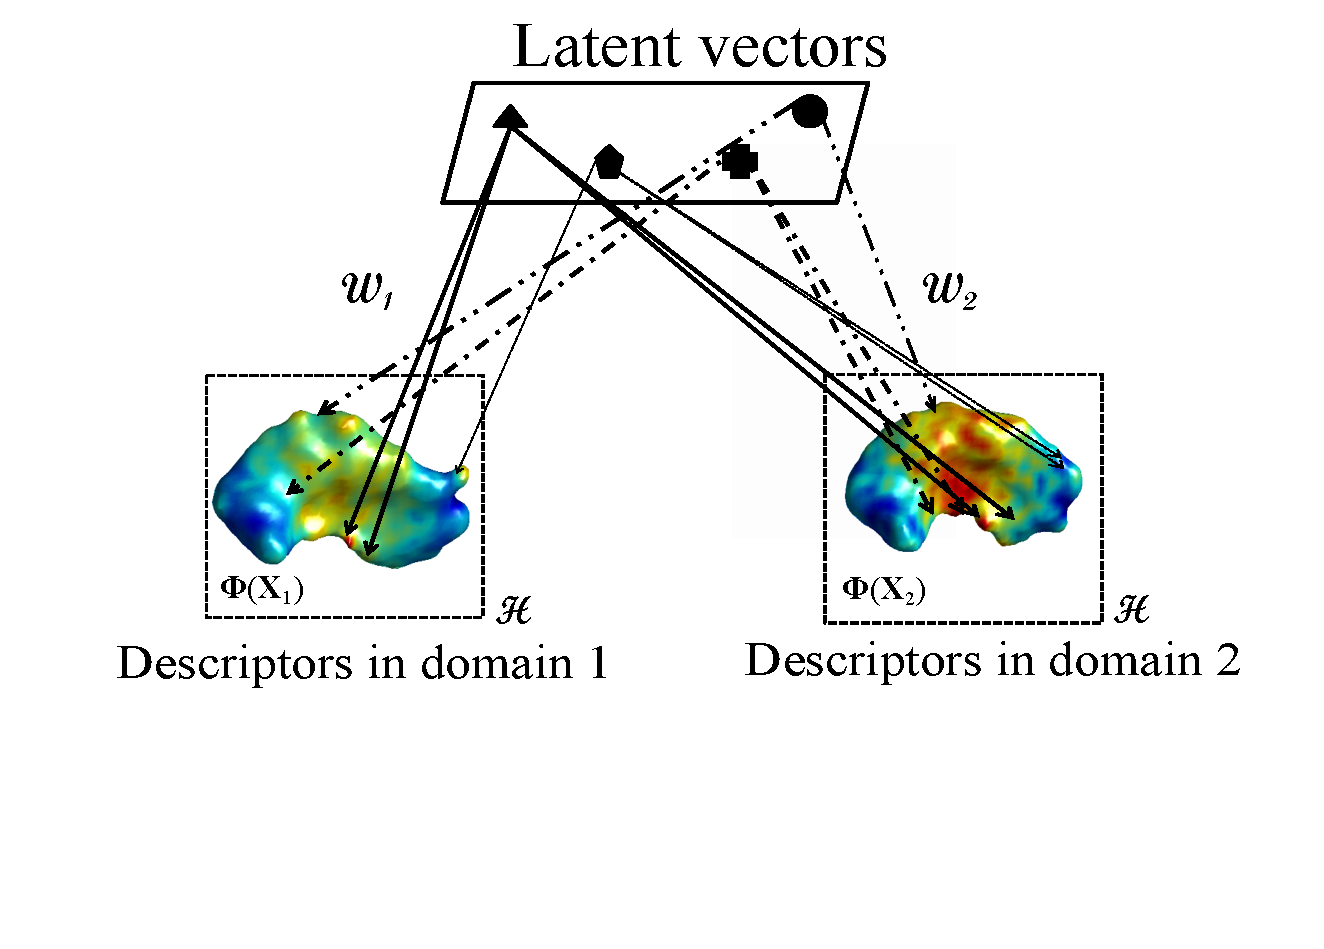
\includegraphics[width=0.4\textwidth]{fig/NLphdModelScheme}
\caption{Scheme for the unsupervised nonlinear clustering method for groupwise correspondence analysis. The
  figure shows an example of establishing clusters of correspondences in Hilbert space for two brain structures (left putamen).}
\label{fig:pipeline}
\end{figure} 

As in \cite{Iwata16}, we use a stick-breaking process to set the mixture weights for a Dirichlet process  with concentration parameter $\gamma$, and then draw the cluster proportions.

The joint probability of the data $\mathcal{X}$, and the cluster assignments $\mathbf{S}=\left\{\left\{s_{dn}\right\}_{n=1}^{N_{d}}\right\}_{d=1}^{D}$ are given by
\begin{equation}
p\left(\boldsymbol{\Phi},\mathbf{S}|\boldsymbol{\mathcal{W}},a,b,r,\gamma\right)=
p\left(\mathbf{S}|\gamma\right)p\left(\boldsymbol{\Phi}|\mathbf{S},\boldsymbol{\mathcal{W}},a,b,r\right).
\label{eq:jointP}
\end{equation}

where $a$,$b$ and $r$ are the hyperparameters.

By marginalizing out the mixture weights $\boldsymbol{\theta}$, $p\left(\mathbf{S}|\gamma\right)$ becomes in
\begin{equation}
p\left(\mathbf{S}|\gamma\right) =\frac{\gamma^{J}\prod\limits_{j=1}^{J}{\left(N_{.j}-1\right)!}}{\gamma\left(\gamma+1\right)\dots\left(\gamma+N-1\right)},
\end{equation}
where $N=\sum\limits_{d=1}^{D}N_d$ is the total number of shape
descriptors, $N_{.j}$ represents the number of descriptors assigned to
the cluster $j$, and $J$ is the number of clusters that satisfies
$N_{.j}>0$.


For our non-linear model, we give the derivation of the likelihood in \eqref{eq:llNLmodel}, in which latent vectors $\Z$ and precision parameter $\alpha$ are analytically integrated out. To this end, we use two mappings functions $\phixnd$ and $\phiwld{j}$, in order to represent our observations and projection matrices in the Hilbert space.

\begin{align}
p\left(\boldsymbol{\Phi}|\Scluster,\W,a,b,r\right) =&\left(2\pi\right)^{-\frac{\sum_d L_d N_d}{2}}r^{\frac{PQ}{2}}\frac{b^{a}}{b'^{a'}}\times \notag\\
&\frac{\Gamma\left(a'\right)}{\Gamma\left(a\right)}\prod_{j=1}^{Q}|\C|^{1/2},
\label{eq:llFinalIntegrallastnm}
\end{align}

Here,

\begin{align}
&a'=a+{\frac{\Sigma_d L_d N_d}{2}}, \notag \\ &b'=b+{\frac{1}{2}}\sum\limits_{d=1}^{D}\sum\limits_{n=1}^{N_d}\kernel{\indobj}{\indobj}-{\frac{1}{2}}\sum\limits_{j=1}^{Q}\boldsymbol{\mu}_j^\top \C^{-1}\muJ,
\end{align}
 and 
\begin{align}
\muJ =\C\sum\limits_{d=1}^{D}{\sum\limits_{n:s_{dn}=j}\kawx}, \quad \quad \C^{-1} =\sum\limits_{d=1}^{D}{N_{dj}\Kaww+r\mathbf{I}}.
\end{align}

where $\kawx$  represents the kernel evaluated in the $\indobj$ objects that has the cluster assignment $j$, $\Kaww$ is the Gramm matrix of the projection matrices for each domain $d$, and $N_{dj}$ is the number of shape descriptors assigned to cluster $j$ in the brain structure $d$ (domain). 

The posterior for the precision parameter $\alpha$ is given by
\begin{align}
p\left(\alpha|\boldsymbol{\Phi},\mathbf{S},\W,a,b\right) = \catD{a'}{b'},
\end{align}
and the posterior for the latent vector $\lvec$ is given by
\begin{align}
p\left(\lvec|\alpha,\boldsymbol{\Phi},\mathbf{S},\W,r\right) = \gD{\muJ}{\alpha^{-1}\C}.
\end{align}

\subsection{Inference}

In order to marginalize out the latent vectors $\Z$, and the precision parameter $\alpha$, we use stochastic EM algorithm \cite{Iwata16}. To this end, collapsed Gibbs sampling for the cluster assignments $\Scluster$, and maximum joint likelihood estimation of the projection matrices $\W$ are alternately iterated.


In the E-step, a new value for $s_{dn}$ is sampled from 
\begin{align}
&p\left(s_{dn}=j|\boldsymbol{\Phi},\mathbf{S}_{\backslash dn},\W,a,b,r,\gamma\right) \propto \frac{p\left(s_{dn}=j,\mathbf{S}_{\backslash dn}|\gamma\right)}{\left(\mathbf{S}_{\backslash dn}|\gamma\right)}\\ \notag
&\times\frac{p\left(\boldsymbol{\Phi}|s_{dn}=j,\mathbf{S}_{\backslash dn},\W,a,b,r\right)}{p\left(\boldsymbol{\Phi}_{\backslash dn}|\mathbf{S}_{\backslash dn},\W,a,b,r\right)},
\end{align}
where $\backslash dn$ represents a value excluding the $n$th
descriptor in the $d$th shape (domain). The first factor in the expression above is
given by
\begin{align}
\frac{p\left(s_{dn}=j,\mathbf{S}_{\backslash dn}|\gamma\right)}{p\left(\mathbf{S}_{\backslash dn}|\gamma\right)}=\left\{ {\begin{array}{*{20}{c}}
   {\frac{N_{.j\backslash dn}}{N-1+\gamma}} & {\text{for an existing cluster}}  \\
   {\frac{\gamma}{N-1+\gamma}} & {\text{for a new cluster}}.  \\
\end{array}} \right.
\end{align}

In the M-step, the projection matrices $\W$ are estimated by maximizing the logarithm of the joint likelihood \eqref{eq:jointP}. The gradient of the joint likelihood is computed by

\begin{align}
&\frac{\partial \log p\left(\boldsymbol{\Phi},\mathbf{S}|\W,a,b,r,\gamma\right)}{\partial\projMat} = \times\Big[\left(-N_{dj}\C\frac{ \partial \mathbf{\hat{K}}_d}{\dWj} \C\right)^\top \times \notag\\
& \sum\limits_{e=1}^{D}\sum\limits_{n:s_{dn}=j} \kawx +\C^\top \sum\limits_{n:s_{dn}=j} \partial\kawx\Big]
\Bigg] \notag\\
& -\frac{1}{2}\sum_{j=1}^{Q}N_{dj} \operatorname{Tr}\left(\frac{ \partial \mathbf{\hat{K}}_d}{\dWj} \C\right).
\end{align}

\section{Results}\label{sec:res}

\section{Conclusions}\label{sec:con}




%\vfill\pagebreak
\section*{Acknowledgments}
This research is developed under the project: \textit{Estimación de los parámetros de neuromodulación con terapia de estimulación cerebral profunda, en pacientes con enfermedad de Parkinson a partir del volumen de tejido activo planeado}, financed by Colciencias with code $1110-657-40687$. H.F. Garc\'ia is funded by Colciencias under the program: \textit{formaci\'on de alto nivel para la ciencia, la tecnolog\'ia y la innovaci\'on - Convocatoria 617 de 2013.}

% References should be produced using the bibtex program from suitable
% BiBTeX files (here: strings, refs, manuals). The IEEEbib.bst bibliography
% style file from IEEE produces unsorted bibliography list.
% -------------------------------------------------------------------------
\bibliographystyle{plain}
\bibliography{bibRevTesisDoc,medImagebib,biblio}

\end{document}
